% #############################################################################
% This is Chapter 3
% !TEX root = ../main.tex
% #############################################################################
% Change the Name of the Chapter i the following line
\fancychapter{Solution Architecture}
\cleardoublepage
% The following line allows to ref this chapter
\label{chap:architecture}

The objective of the system was to develop a device in a box format to enable users to establish safe channels of communication. This is achieved with a safe and secure device which is personal to each individual. In order to secure the communications between users, the device saves the user's sensitive data, such as keys, and performs all security critical operations.
The system is designed so that each user has it's own physical box.

% -----------------------------------------------------
% -----------------------------------------------------
\section{Components} \label{chap:arch:components}

%% Insert image "figure"
\begin{figure}[h]
    \centering
    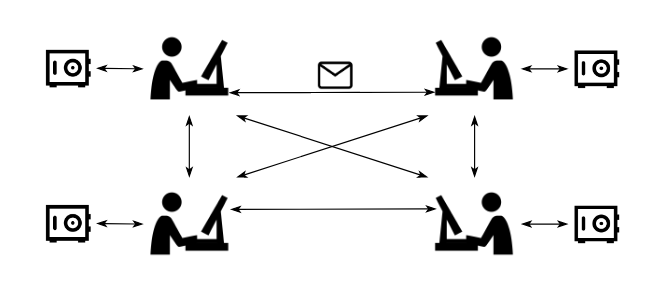
\includegraphics[width=0.5\textwidth]{./Images/main-figure.png}
    \caption{Client and device}
    \label{fig:main-system}
\end{figure}

The solution is composed of two main components, as shown in figure \ref{fig:main-system}:

\begin{itemize}
    \item The physical box which responsible for securing communications;
    
    \item The client application on the user's computer which provides an interface for the user to execute operations on the box.
\end{itemize}

By separating these components, the security of the system is isolated and solely of total responsibility of the box. It is not dependent on the user's personal computer.

Both components are connected through a common interface, such as USB, in order to be more easily accessible to the end users.

Figure \ref{fig:securebox} depicts the client application, interacting with the secure device through the application programming interface (API), the implementation of operations inside the device and secure storage where all the keys are stored.
%% Insert image here
\begin{figure}[h]
    \centering
    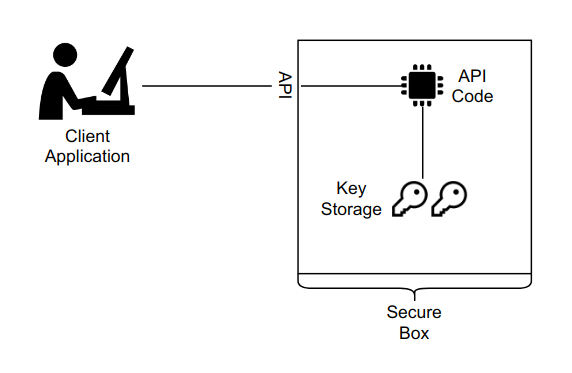
\includegraphics[width=0.5\textwidth]{./Images/securebox.png}
    \caption{Client application and secure device}
    \label{fig:securebox}
\end{figure}


% -----------------------------------------------------
% -----------------------------------------------------
\section{Operations} \label{chap:arch:operations}

The system operations will ensure the system requirements and services are fulfilled.
For the user to be able to execute them, he first must authenticate himself to the device. This is done with a PIN or password, which identifies the user. Once authenticated, the operations will be available to the user to be executed in the box.

The operations are split in three types:
\begin{itemize}
    \item The administration operations manage the authentication and communication configuration;
    \item The message exchange operations secure the user's communication;
    \item The key exchange operations manage the keys stored inside the device, which will be used to secure communications.
\end{itemize}

% -----------------------------------------------------
\subsection{Administration Operations} \label{chap:arch:ops:administration}

The administration operations will allow the user to manage the authentication related parameters.
The only operations of this type is to change the authentication PIN. The device will be initialized from fabric with a default PIN which must be supplied to the user. Before performing any operation the user should change his PIN to begin secure communications.

% -----------------------------------------------------
\subsection{Message Exchange Operations}  \label{chap:arch:ops:message}

The main operations will be responsible to secure the communications between users. These operations will fulfill the confidentiality, authentication and non-repudiation services.

\begin{itemize}
    \item Secure message exchange with confidentiality and authentication. The objective of this operation is to send and receive messages to and from the device. Plaintext messages will be returned to the user encrypted and authenticated with their key stored inside the device. In the case of encrypted and authenticated messages, an error will be returned if the decryption was unsuccessful, otherwise, the user will receive the plaintext message;
    \item Digital Signature operation will provide non-repudiation to a message. The user will send a message to the box, and the subsequent signature will be returned, which can be used to verify the message authorship. To verify a signature, the user sends it to the device, and receive the appropriate message, success or failure to verify.
\end{itemize}

% -----------------------------------------------------
\subsection{Key Exchange Operations}  \label{chap:arch:ops:key}

These operations will handle key exchange when new keys need to be generated and exchanged between users, to enable further communications, and to import other user's public keys. This will serve the secure storage and key management services.

The first operations will enable the user to ask for a new key, generated inside the box, in order to securely send it to another user. The user receiving the new key, generated by another user, will receive and store the key inside the box.
The final operation will provide a way to import other user's public keys, as well as export their personal public key, to be shared with another user.


% -----------------------------------------------------
% -----------------------------------------------------
\section{The Solution in depth}  \label{chap:arch:solution}

Symmetric keys will be used to encrypt and authenticate messages. They have better performance with larger messages compared to asymmetric keys. Each user can have stored in their box, several symmetric keys. This enables the user to establish secure communications with multiple different people or groups.
The non-repudiation property of asymmetric keys will be used to create digital signatures of documents. The other use, will be to share symmetric keys between user who wish to communicate. The box stores the private and public key pair of the user, and the public keys of people the user wishes to trade secrets with.

\section{Initial State} \label{chap:arch:initial-state}

The users will receive the device with a pair of private and public keys, generated inside the device from fabric. Each device will have the user's public keys, whom he wishes to communicate. The user can request whose public keys he wants, before the device is initialized in fabric. This allows the users to trade symmetric keys between them, which they can user to begin trading messages securely. In addition, the device can also come with a symmetric key stored in each the user's device.

When a new user wants to establish secure communications with an existing user or a group, he must share his public key with the user, ideally physically to ensure there are no mistakes or attacks. After this they can securely share symmetric keys to enable efficient and secure messaging.

% -----------------------------------------------------
% -----------------------------------------------------
\section{Protocol} \label{chap:arch:protocol}

A protocol was devised for every operations with different phases and data for each operation.

% -----------------------------------------------------
\subsection{Authentication Protocol} \label{chap:arch:protocol:auth}

%% Insert protocol image here
\begin{figure}[h]
    \centering
    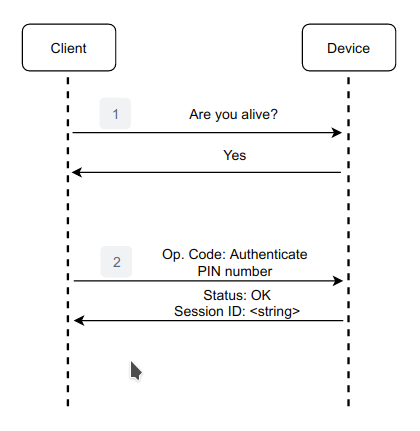
\includegraphics[width=0.5\textwidth]{./Images/authentication.png}
    \caption{Authentication Protocol}
    \label{fig:protocol:authentication}
\end{figure}

Before executing any operation the user must authenticate himself to the device.
\begin{enumerate}
    \item The first phase is initiated by the user by sending a message to check if the box is alive and connected to the computer.
    \item The operation will move to the second phase when the user receives an affirmative response. He will then send the operation code, which indicates he wants to authenticate himself, and the authentication PIN. The device will respond with a status parameter indicating failure or success. When successful the box will also return a session ID string, which the user will need for further operations, to prove he has authenticated himself.
\end{enumerate}

%% TODO - in case I decide to keep the session ID, add paragraph explaining how it's used in all operations, else delete this

% -----------------------------------------------------
\subsection{Administration Protocol} \label{chap:arch:protocol:admin}
%% Insert protocol image here
\begin{figure}[h]
    \centering
    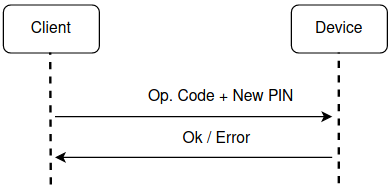
\includegraphics[width=0.5\textwidth]{./Images/change-PIN.png}
    \caption{Change Authentication PIN protocol}
    \label{fig:protocol:change-PIN}
\end{figure}

As explained before, there is only one administration operation, changing the authentication PIN, pictured in figure \ref{fig:protocol:change-PIN}.

The user initiates by sending the operation code, identifying the operation, the new PIN number and the session ID acquired previously. The device verifies the session ID and send a response, indicating the success or failure of the operation.

% -----------------------------------------------------
\subsection{Message Exchange Protocol} \label{chap:arch:protocol:message}

%% Insert protocol image here
\begin{figure}[h]
\centering
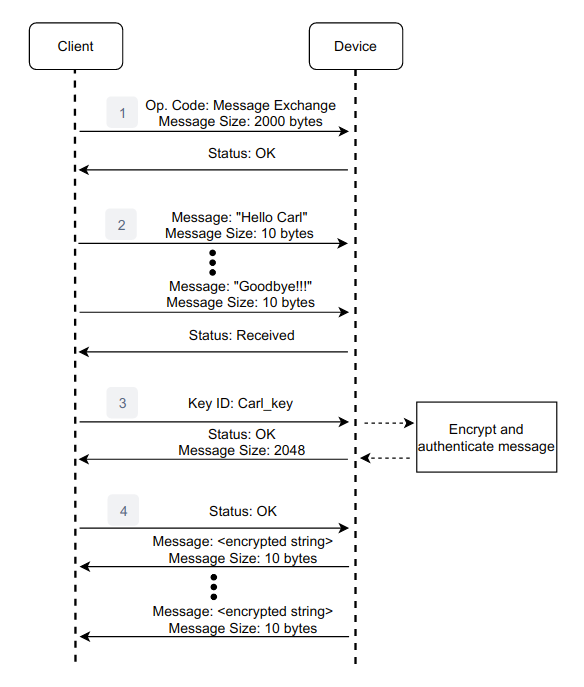
\includegraphics[width=0.6\textwidth]{./Images/message-exchange.png}
\caption{Message Exchange Protocol}
\label{fig:protocol:message-exchange}
\end{figure}

Protocol to encrypt and authenticate messages:
\begin{enumerate}
    \item The user sends the operation code, signaling he wants to send a message, and the message size;
    \item The box will respond with an OK message that the user can begin transmitting the message. The message will be transmitted a maximum of X bytes per "packet". Each packet contains the message information and the size of the message information for that packet. When the transmission ends, the device will confirm the reception;
    \item The user subsequently will respond with the symmetric key ID, which he wants to encrypt and authenticate the message with. The box will handle the cryptographic operations and return a status message and the encrypted message size.
    \item After the client confirms, the encrypted message with the additional MAC and IV parameters appended, will be returned in the same manner it was sent.
\end{enumerate}

Protocol to decrypt and verify message authentication:

\begin{enumerate}
    \item The operation code is sent, as well as the encrypted message size;
    \item The box will respond with an OK message that the user can begin transmitting the message, one packet at a time;
    \item When the message transmission ends, the device will confirm its reception, and the user will subsequently respond with the symmetric key ID, which can decrypt and verify the message authentication;
    \item After performing the decryption and authentication operations, the device will return a message indicating its success or failure. In case of a successful operations, it will return, in the same manner it was sent, the plaintext message.
\end{enumerate}

In the case of digital signatures, the user's must have each others public keys, if they do not already have them.
%% -------
Protocol for generating a digital signature:
\begin{enumerate}
    \item The user initiates with the code operation and the plaintext message size;
    \item When the box responds with an OK message, the user transmits the message one packet at a time;
    \item In possession of the message, the device will generate the digital signature using the user's private key. When finished the signature is sent back.
\end{enumerate}

Protocol for verifying digital signatures:
\begin{enumerate}
    \item The user initiates with the code operation;
    \item When the box responds with an OK message, the user transmits the message one packet at a time;
    \item When done, the user also sends the signature and the name of the signer, so the device knows what public key to use to verify the signature;
    \item Then, the device will verify the digital signature using the signer's public key, message and signature. The result will be sent back to the user.
\end{enumerate}

% -----------------------------------------------------
\subsection{Key Exchange Protocol} \label{chap:arch:protocol:key}
%% Insert protocol image here

Protocol to import public keys:
\begin{enumerate}
    \item The user send a message with the operation code, indicating he wants to send someone's public key;
    \item After the device responds with an OK signal, the user sends the public key, and the name of the owner of the public key;
    \item The device then informs the user of the operation's success or failure.
\end{enumerate}

%% -------
Just like digital signatures, for users to be able to share symmetric keys between each other, they must possess each others public keys in their device. If not, they must physically meet to share them, and import them to their respective devices, with the available operation.

Protocol to send new symmetric key:
\begin{enumerate}
    \item The user sends a message with the operation code;
    \item After the device responds with an OK signal, the user sends the key ID, the name the key will be saved as, and the name of the user he wants to share the key with, so the device knows which public key to use to secure the key;
    \item A new symmetric key will be generated and saved in the device's secure storage, with the key ID sent by the user. The box will encrypt and sign the key with public-key cryptography, and send it to the user, which he can securely share with the other user.
\end{enumerate}

Protocol to save new symmetric key, received from another user:
\begin{enumerate}
    \item The user sends a message with the operation code;
    \item After the device responds with an OK signal, the user sends the key ID, the name of the key sender, and the encrypted and signed key;
    \item The device will then verify the signature with the sender's public key and decrypt the key, subsequently saving it in the device's secure storage along with other keys already present.
\end{enumerate}
